
\documentclass[preprint,12pt]{elsarticle}

\usepackage[spanish]{babel}
\usepackage{amssymb}
\usepackage{graphicx}
\usepackage{lineno}
\usepackage[utf8]{inputenc}
\usepackage{url}
\usepackage{natbib}

\begin{document}
	
	\begin{frontmatter}

		\title{\huge  Laboratorio 02: Qlik	 }
		\author{	Tarqui Montalico,Risther(2017057469)}
		
		





\end{frontmatter}

%%INICIO Resumen
\section{Objetivo}
	
	Comprender el funcionamiento de Qlik realizando un ejercicio con intrucciones precisas.
%%FIN Resumen


%%INICIO Introducción
\section{Desarrollo}

	\begin{itemize}
			\item Develop a sheet using the ‘Insight advisor’ \\
		 		
		 		
		 		\\Create a new app
		 		\\• Launch Qlik Sense. \\
		 			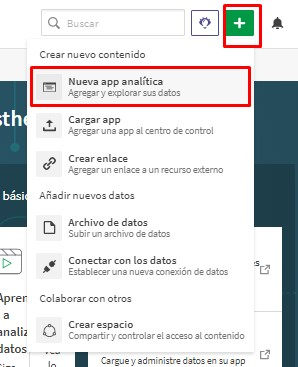
\includegraphics[width=7cm]{./IMAGENES/1.1} \\
		 		\\• Create a new app.
		 			o Name the app: “My Sales Analysis”.
		 			Create and Open app.
		 		
		 		 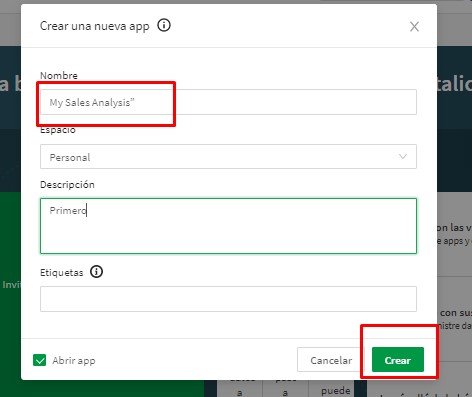
\includegraphics[width=10cm]{./IMAGENES/1.2}  \\
		 		 
		 		 \\Load data  \\
		 		\\• Use the Add data from files and other sources tile in order to add the
		 		Excel data to the app (from the file ExerciseData.xlsx).
		 		o Load all fields from the spreadsheet, by clicking the Add data
		 		button. \\
		 		 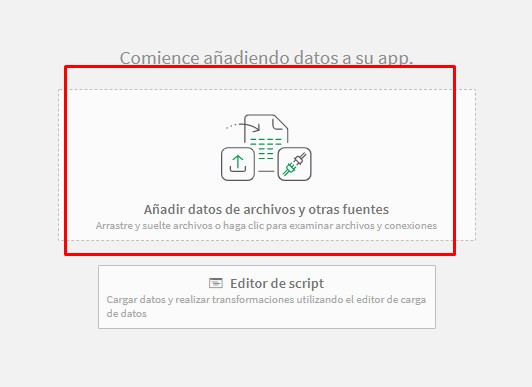
\includegraphics[width=10cm]{./IMAGENES/1.3} \\
		 		 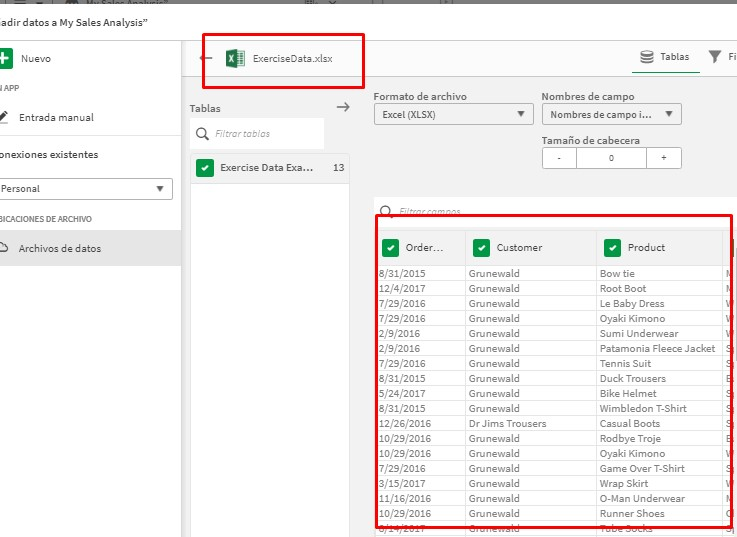
\includegraphics[width=10cm]{./IMAGENES/1.3.2} \\
		 		\\Review data
		 		\\• Use the quick access menu to navigate to the Data manager view, in
		 		order to learn more about this table.
		 		
		 		 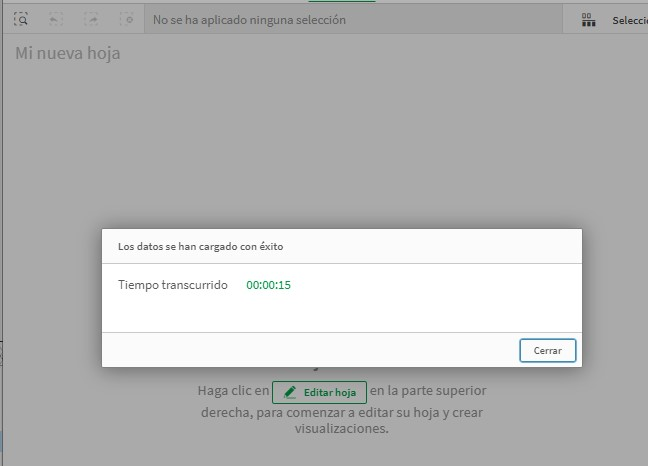
\includegraphics[width=10cm]{./IMAGENES/1.4}
		 		\\• Open the Data manager’s table editor view by clicking on the icon
		 		along the bottom of the view.
		 		Click on the indicated fields and view the summary card to answer the
		 		following questions:
		 		o How many distinct 
	 				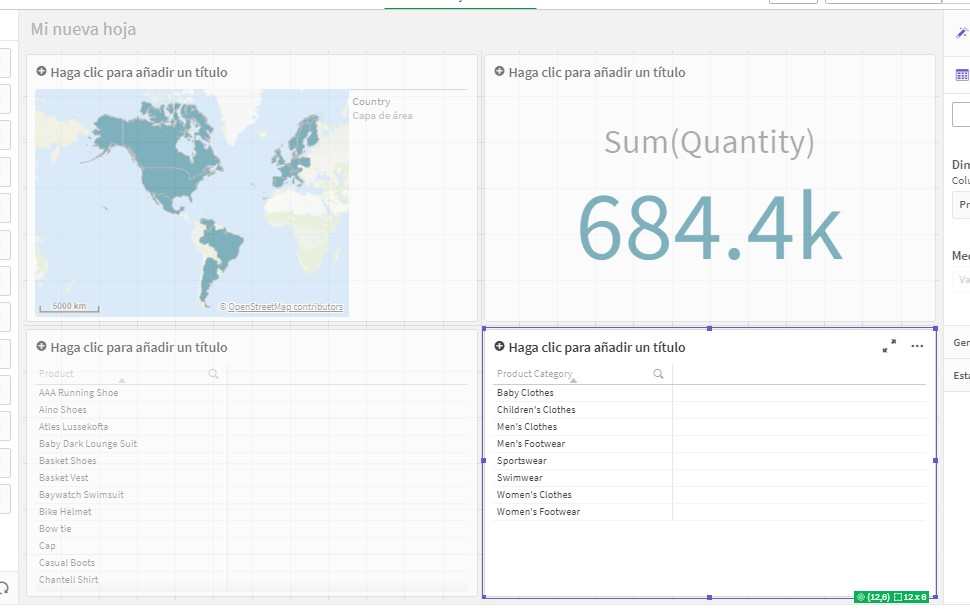
\includegraphics[width=7cm]{./IMAGENES/1.5}
	 				
	 		\\ \item Develop a sheet using ‘Chart suggestion assistance’ \\
	 		
	 			\\ • Use the quick access navigation submenu under Analyze > Sheet to select Insights, click the button to  \\
	 			 \\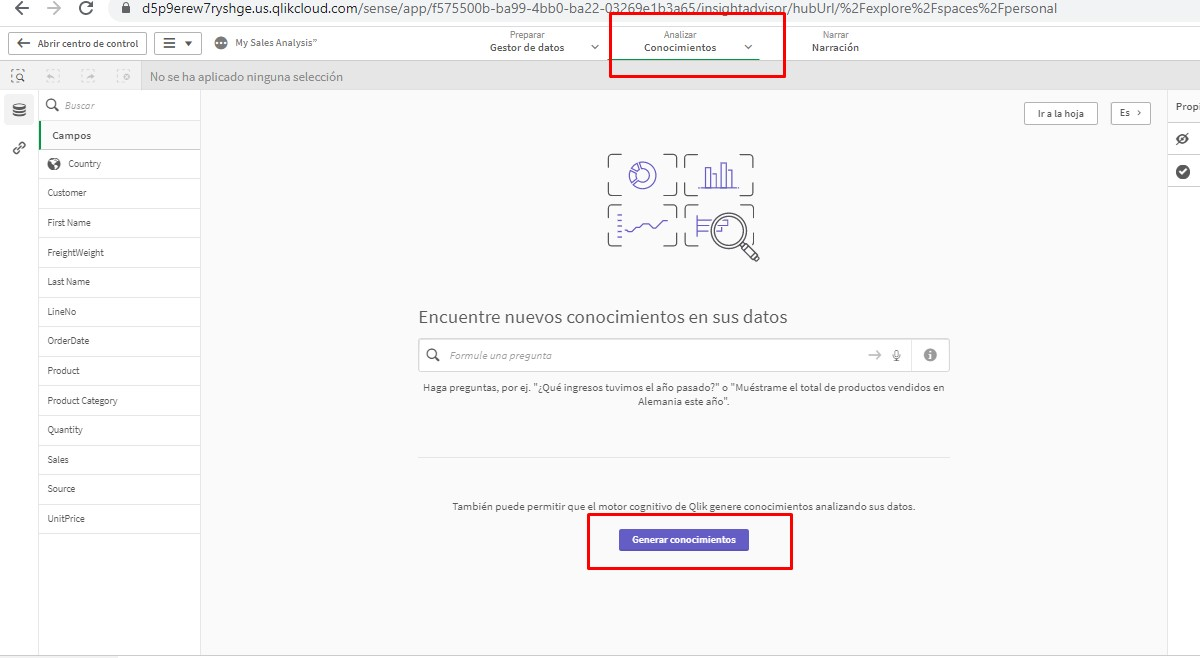
\includegraphics[width=10cm]{./IMAGENES/2.1} \\
	 			Generate insights - based upon the entire data model.
	 			\\ • Locate the map in the list of proposed charts, and Add to sheet > My new sheet. \\
	 			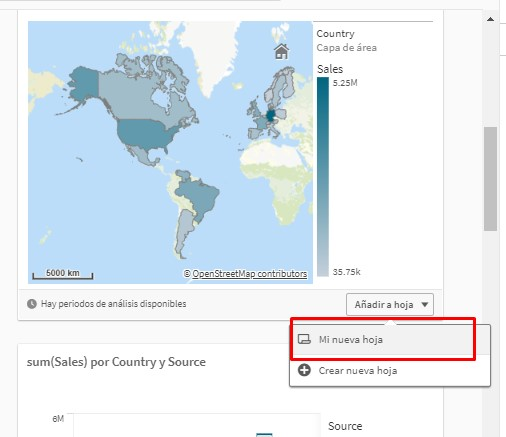
\includegraphics[width=10cm]{./IMAGENES/2.2} \\
	 			\\ • Use the panel along the left to select (checked boxes) the fields: Product and UnitPrice.
	 			o Locate the bar chart titled: sum(UnitPrice) by Product, and Add to sheet > My new sheet.
	 			o Clear the fields ( ).
	 			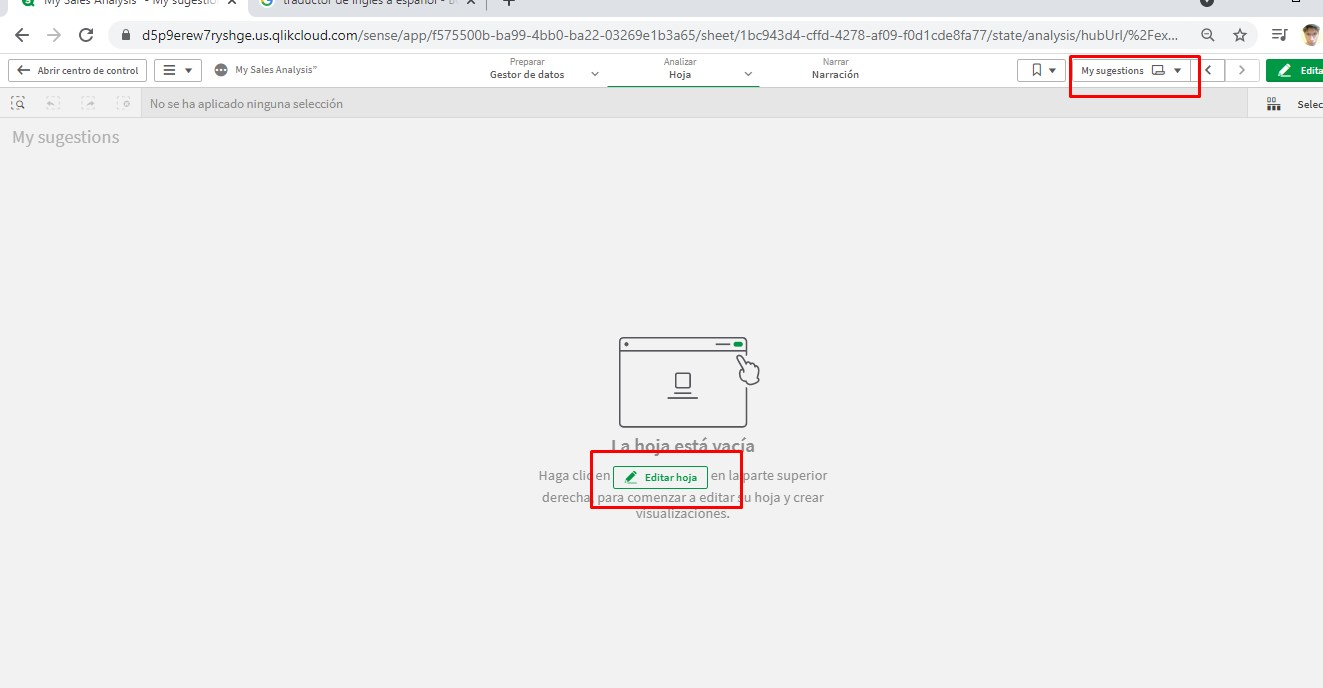
\includegraphics[width=10cm]{./IMAGENES/3.1} \\
	 			\\ • Type the following into the ‘Ask us a question’ field: Which country has highest quantity? (and submit
	 			question).
	 			o Locate the bar chart titled: sum(Quantity) by Country, and Add to sheet > My new sheet.
	 			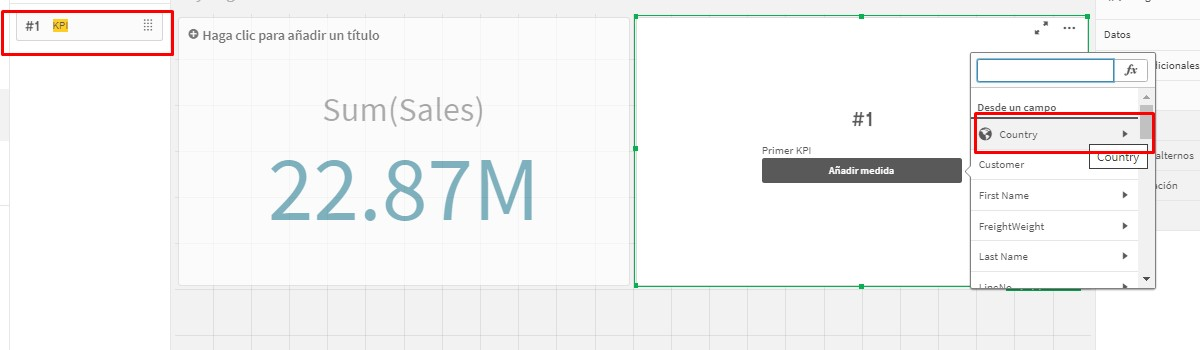
\includegraphics[width=10cm]{./IMAGENES/3.2} \\
	 			\\ • Use the quick access navigation submenu under Analyze > Insights to select Sheet, and evaluate the
	 			sheet you have created. It should appear as you see below:  \\
	 			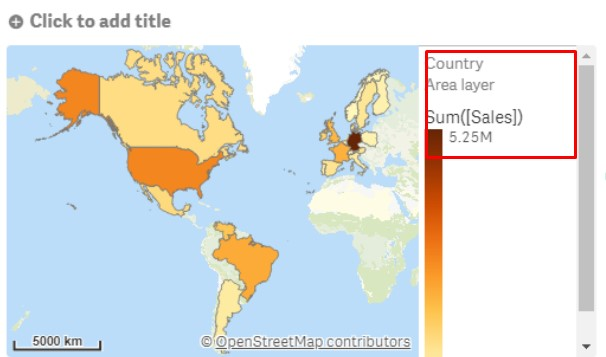
\includegraphics[width=10cm]{./IMAGENES/3.3}
 \\
	 		\item Develop a sheet using ‘Chart suggestion assistance’ (cont’d) \\
	 			\\ Use the sheets drop down menu ( ) to Create new sheet.
	 			o Title the sheet: “My suggestions“.
	 				
	 					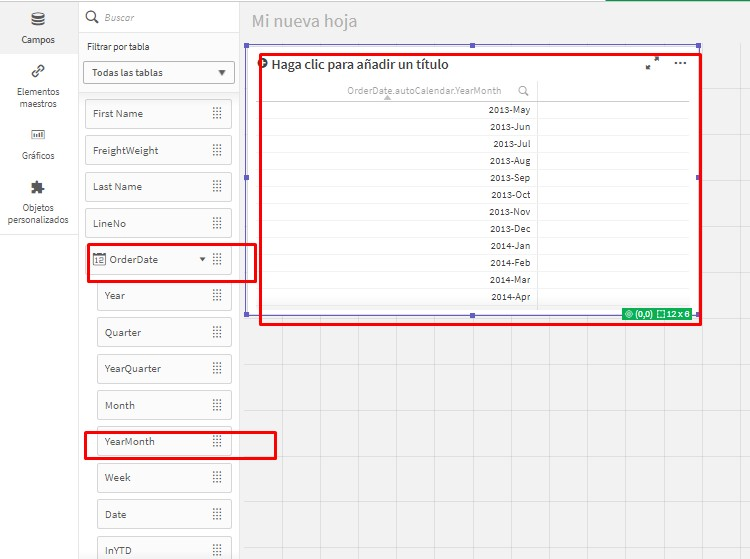
\includegraphics[width=10cm]{./IMAGENES/4.1} \\
	 			
	 			\\ In Edit sheet mode, use the Fields ( ) section of the assets panel, drag & drop the Sales field onto
	 			the visualization area.  \\
	 					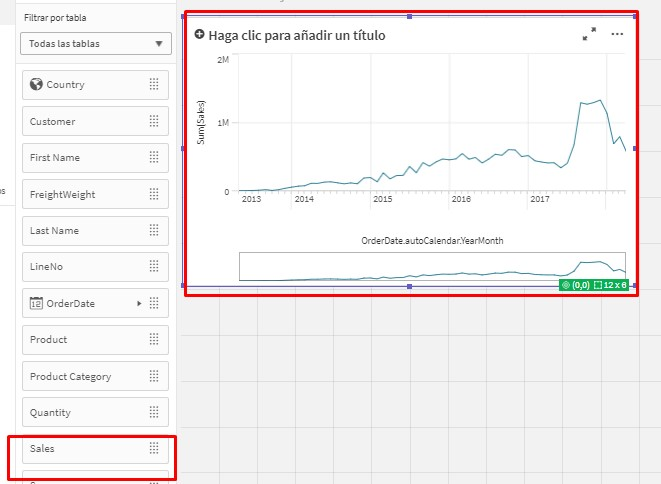
\includegraphics[width=10cm]{./IMAGENES/4.2} \\
	 			\\ Drag & drop the Country field onto the KPI chart, ensuring that the ‘ghost’ image covers the entire
	 			chart.   \\
	 				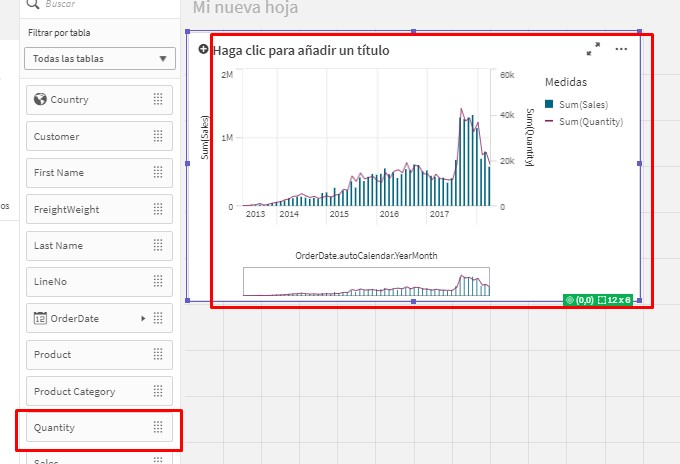
\includegraphics[width=10cm]{./IMAGENES/4.3} \\ \\
	 		\item Try an alternate suggested chart type \\
	 				 \\
	 			\\ Return to Edit sheet mode and consider alternative chart suggestions. 
	 				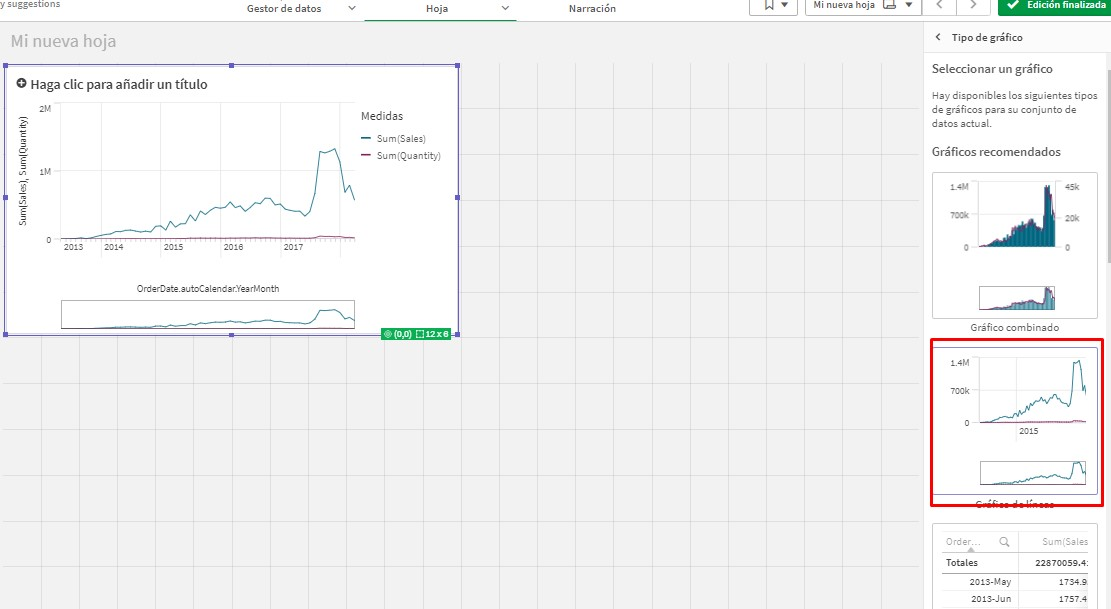
\includegraphics[width=10cm]{./IMAGENES/5.1}
	 		\item Toggle the Chart suggestions switch from ‘on’ to ‘off’
	 		
	 			\\ Notice that the properties panel for the charts configured with assistance present only limited settings
	 			options for you to adjust  \\
	 				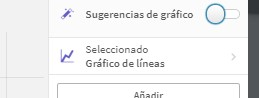
\includegraphics[width=10cm]{./IMAGENES/6.1}
	 			\\ We would like to adjust the color scheme applied to the country shapes on the map chart, so toggle the
	 			Chart suggestions switch to ‘off’.
	 			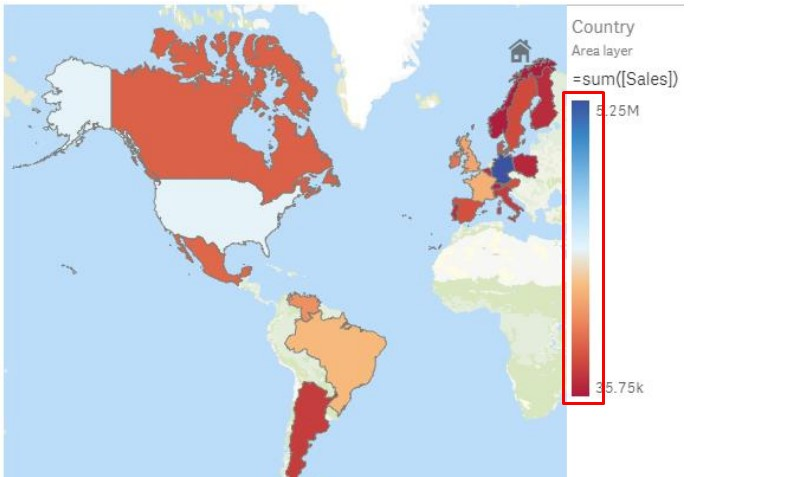
\includegraphics[width=10cm]{./IMAGENES/6.2}
	 			\\ The resulting map should appear as you see below.
	 		\item Develop a sheet without assistance \\
				
				\\ Create a new sheet in the app, titled “My custom charts“.  \\
				  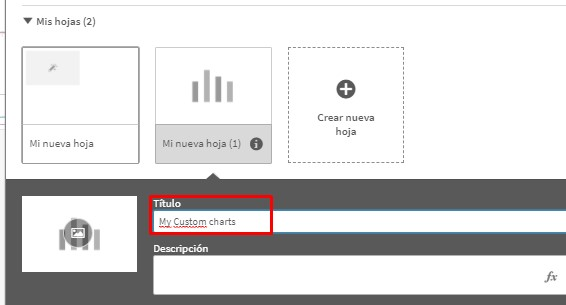
\includegraphics[width=10cm]{./IMAGENES/7.1}
				\\ Drag & drop objects from the Charts ( ) section of the assets panel to the visualization area, and
				resize each, to populate a sheet with a Bar chart, Table, Pie Chart, KPI, Filter pane, and Text &
				image area organized within the visualization space as shown below:
				
	 				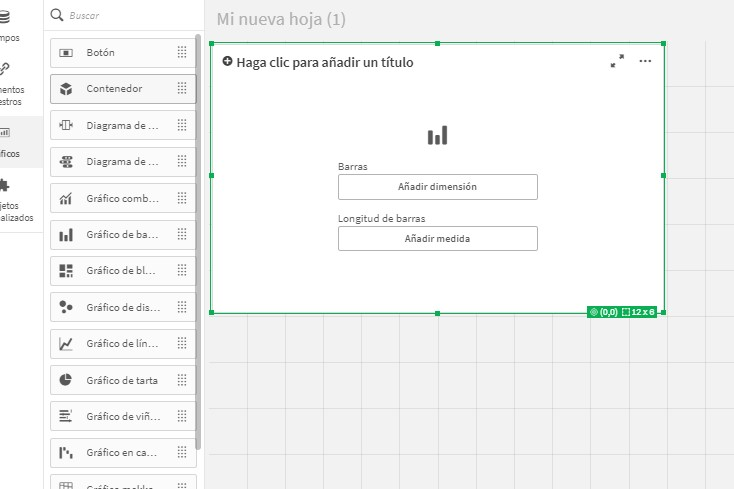
\includegraphics[width=10cm]{./IMAGENES/7.2}

			\item Develop a sheet without assistance (cont’d)\\
				\\ The sheet you configured should appear as you see below:  \\
					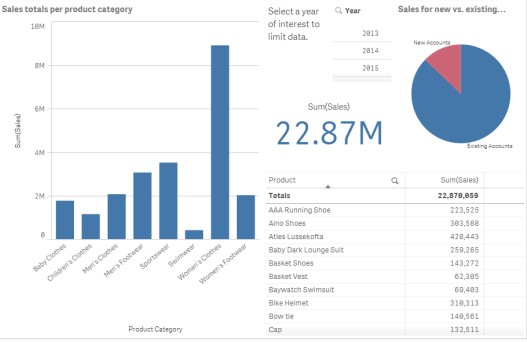
\includegraphics[width=10cm]{./IMAGENES/8.1}
			
			\item Tell a story\\
				\\ • Use the quick access menu to navigate to the Storytelling view.
				
					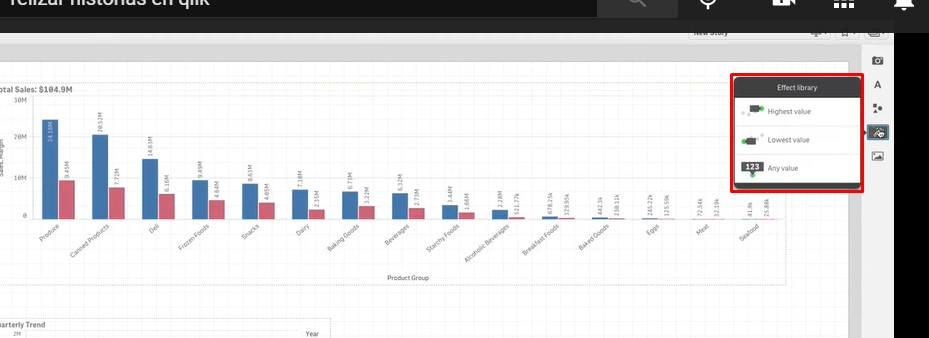
\includegraphics[width=10cm]{./IMAGENES/9}
				\\ • Use the Snapshot library ( ) to add the two snapshots you took to the blank slide.
				\\ • Use the Text library ( ) to add a label for 2013 (to the pie chart with the smaller New Accounts
				wedge).  \\
					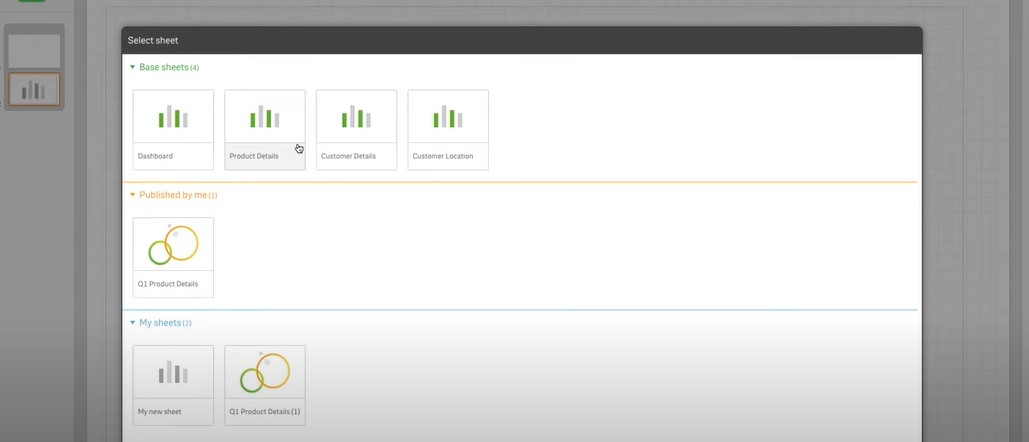
\includegraphics[width=10cm]{./IMAGENES/9.1}  \\
				\\ • Add another label for 2015 (to the pie chart with the larger New Accounts wedge).
				
					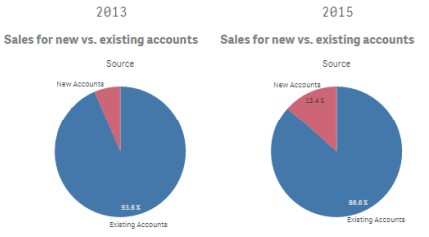
\includegraphics[width=10cm]{./IMAGENES/9.2}
				\\ • Use the Sheet library ( ) to add the sheet titled My suggestions to a slide in the story.
				\\ • Play the story ( ). Click on different visual aspects of your live data sheet (like individual country
				shapes) in order to see that it is an interactive slide.  \\
				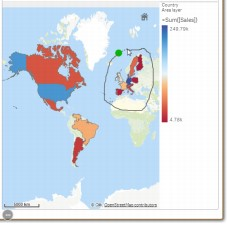
\includegraphics[width=10cm]{./IMAGENES/9.3}
	 
	\end{itemize}
%%FIN Introducción

		


\section{Conclusiones}
		\begin{itemize}
		\item Qlik es muy bueno con el filtro de datos,porque ya tiene definido elementos. Cuando cargamos datos, en este caso uno de excel, los lo une con sus elementos ya definidos para que podamos trabajar en el analizis de datos.
		\end{itemize}
\section
%%----------------------------------------------------------------------------------------------------------------------------------------------------------
%%FIN Marco Teórico




%CONCLUSIONES







	
	
%\citep{referenciarobles2}  


\end{document}

